\clearpage
\section{Introduction : The Ludicrous Fiction of Innovation}

\bigskip

The \textit{Junkware }installation offers a grotesque representation of
the actual innovation process. We recycle existing patents data and mix
it with biometrics information gathered from the audience to generate
textual and visual representation of futuristic objects. This
speculative machine is introduced as a groundbreaking technology
developed by fictional characters representing a scientific team. Setup
as a mobile lab, we invite the audience to reflect on the impact of
their fascination for science and technology in our innovation theater.

China


\bigskip

In this paper, we will first introduced the data and routines we used to
generate visual and text for our fictional objects. The second part
will provide a detailed description of the characters and whereabouts
of the play. The third part will describe the stage and setup of the
installation itself, including costumes and accessories. Finally, we
will discuss about the actual observations of what can been seen a a
social experiment. We will show how digital art could benefit by
incorporating human performances and being displayed in trivial
context. We will conclude on the interest for art, technology and
science to represent itself.


\section{From design thinking to junk-production}
\subsection{Design thinking and its failure facing future times }
The \textit{Junkware} project originates in the creation of a
collaborative methodology to enable teams in France and China to design
together fictional objects from a distant future. Initially conceived
as a sequence of workshops, the process of imagining solutions for a
non-existing world quickly faced numerous issues. First, to lead a
workshop with teams evolving in different languages, cultures and even
time(zones) was challenging us practically. Design thinking [Adler2011]
had already try to tackle those issues with different degrees of
success by using a problem-solving approach to specific question. 


\bigskip

Here though, our major problem was the lack of specifics about problems
that may arise in a future time, and therefore the absence of need for
solutions to non-existing problems. The difficulty to anticipate
problems was unveiling our inability to provide common ground for very
different teams to collaborate. To solve this practical issue, we were
facing the biggest paradox of innovative design : obsolescence. Is
design really stuck in the present ? Should design intentionally ignore
the future to exist ? A great rush for innovative products is pushing
us towards an urgent necessity of practicing design. But should we
design before having identified common problems ? Furthermore, has
defining problems become the role of design ?


\bigskip



\begin{center}
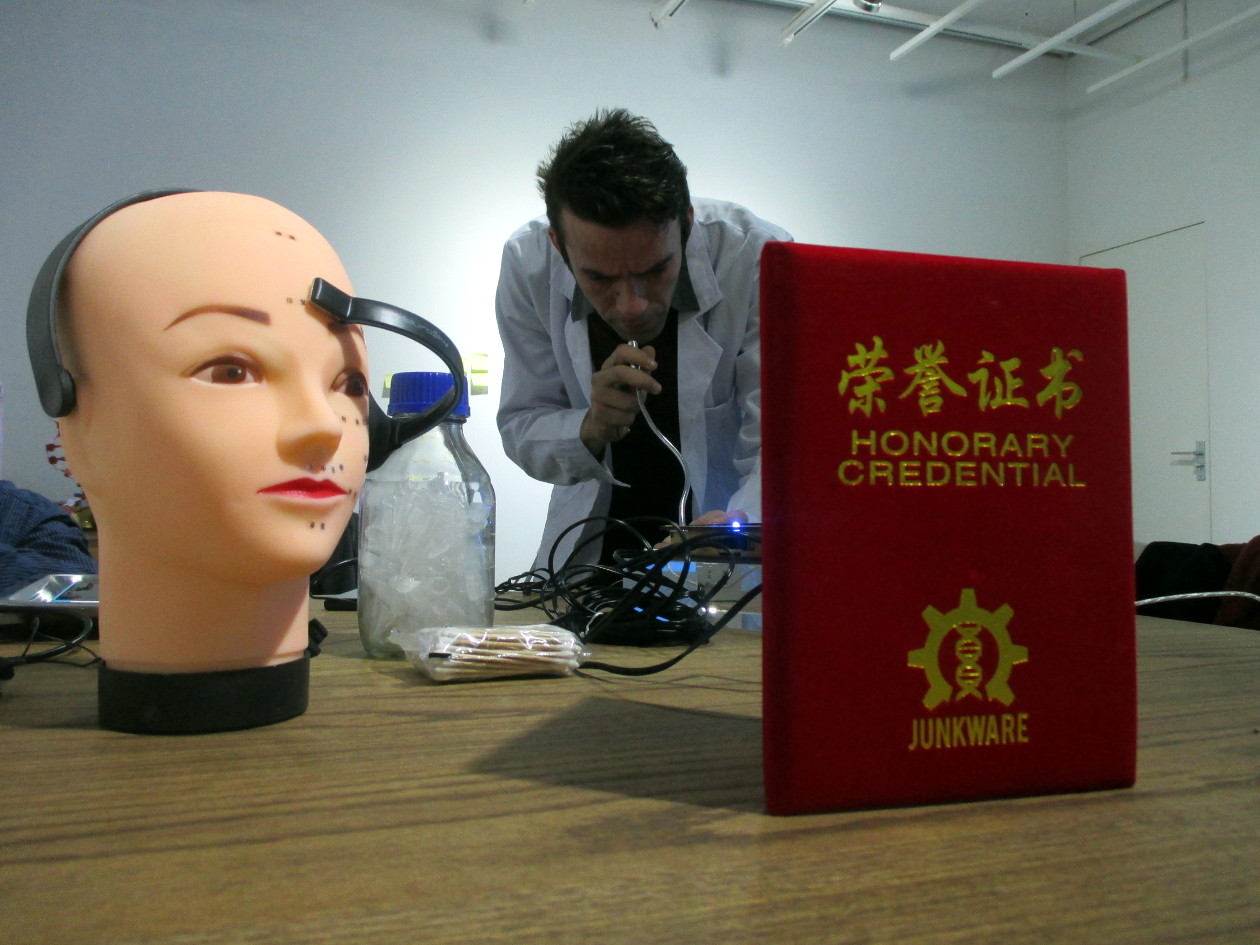
\includegraphics[width=3.8083in,height=2.8563in]{images/junkware-img1.jpg}
\end{center}
{\centering
Caption : The Pr. Lafleche is calling the audience to come and take the
experiment. 
\par}

{\centering
Credits : Junkware (CC)
\par}

\subsection[Junkware : Obsolescence ]{Junkware : Obsolescence }
The vertiginous increase in research, design and production capacity of
the last 20 years has lead most technological industries to adopt quick
and short product cycles. Planned obsolescence has therefore become a
prominent component of design in order to adapt products to the quick
evolution of technology and markets [Grout2005]. Market studies for
technological products have been largely based on consumers behaviors,
making the act of buying a final and decisive goal. Large industrial
sectors have oriented their marketing towards this short-term cognitive
process (\textit{call to action}) [Perry2004] to bring into business
quickly-designed and short-living products. This has supported the
appearance of an unprecedented stock of objects, with for instance an
average number of 1.3 cell phone per inhabitant on earth [5].


\bigskip

In his book \textit{Junkware},\textit{ }Bardini investigates the role of
what he called \textit{j}\textit{unk} : {\textquotedblleft}\textit{Junk
is what has been used with fervor and remains because of this
fervor.}{\textquotedblright} [Bardini2011] He starts by investigating
the \textit{junk-}\textit{DNA} that supposedly makes 98.5\% of the
human genome without fulfilling any proper genetic function. Then he
discuss about junk-food, junk-mail and the piles of junk that are
piling up in our garages and states : \textit{{\textquotedbl}most of
culture and nature, including humans, is composed of useless, but
always potentially recyclable, material otherwise known as
{\textquoteleft}junk.{\textquoteright} {\textquotedbl} }[Bardini2011].
Beneath the obvious danger of accumulation stands an opportunity for
objects to find their own future. And what about us ? Have we also
become the junk of a bigger innovation planning \ ?


\bigskip

{\bfseries
China and the speculative development }

{\bfseries
\textmd{The }\textmd{\textit{Junkware}}\textmd{ }\textmd{project
}\textmd{ha}\textmd{ve}\textmd{ been }\textmd{created }\textmd{in
mainland China}\textmd{, more specifically in }\textmd{the city of
}\textmd{Shanghai}\textmd{. }\textmd{We have shortly introduced how
th}\textmd{e creation of link}\textmd{s}\textmd{ between }\textmd{both
teams in }\textmd{France and Chin}\textmd{a}\textmd{ }\textmd{have
contributed to }\textmd{our shift in purpose and methodology.
}\textmd{China }\textmd{also }\textmd{offers a very typical
}\textmd{setup when it comes }\textmd{to reflection about }\textmd{the
}\textmd{future }\textmd{and the production of }\textmd{technology.
}\textmd{For last 30 years, }\textmd{the
}\textmd{\textit{{\textquotedblleft}made in China{\textquotedblright}
}}\textmd{ha}\textmd{ve}\textmd{ }\textmd{b}\textmd{een }\textmd{the
}\textmd{core }\textmd{engine }\textmd{of }\textmd{the production of
}\textmd{most }\textmd{technolog}\textmd{ical devices and assets
}\textmd{worldwide}\textmd{. }\textmd{This }\textmd{industrial
}\textmd{develop}\textmd{ment}\textmd{ }\textmd{has
br}\textmd{ou}\textmd{g}\textmd{ht}\textmd{ }\textmd{to }\textmd{China
}\textmd{not only }\textmd{extended}\textmd{ }\textmd{knowledge
}\textmd{and skills in }\textmd{manufacturing }\textmd{but also
}\textmd{enormous }\textmd{design }\textmd{capacity }\textmd{of a new
kind }\textmd{[}\textmd{Dantec2012}\textmd{]. }}


\bigskip

The region of the Pearl River Delta hosts today the largest production
facility cluster in the world, with quasi-unlimited access to cheap,
fast and incredibly diverse offer of manufacturing services. The
ability of building products very quickly at a very low-price has first
lead to the creation of an economy of cheap counterfeit goods
(\textit{shanzhai}). The increasing availability of
{\textquotedblleft}white box{\textquotedblright} kits and ready-to-use
designs [Chien2010] has brought new dynamics to the creation of
electronics products : a general model can now be modified through very
fast iteration. Subsets of existing products are being merged through
small changes to a general models. Features that were once proper to a
large rande of products end up being hybridized very easily into a
single model. In \textit{Junwkare, }we used the patent database to
represent this generative dynamic that creates new models from a set of
existing features. All the costumes, furniture and accessories were
also bought on the Chinese website \textit{Taobao }that hosts the
largest database of cheap and unexpected manufactured products ever
seen.


\bigskip

In this context, the future evolutions are generated and therefore can
be entirely defined by detailed processes and parameters. The strategic
panic induced by constant mutations and changes can be turn into an
advantage through the \textit{{\textquotedblleft}}\textit{pragmatic
explo}\textit{i}\textit{tation of randomness{\textquotedblright}
}[Koolhaas2000]. Newness become the result of the daily accidents,
expected lands of opportunities in the plan. While the speculative
system of communist China was justifying today{\textquotesingle}s
endeavors with remote goals, the generative model uses the absence of
defined roadmap as an excuse to postpone the reward. Always
perfectible, present meets future ends at each second under the form of
a draft or a simulation. Speculation sustains itself with future
values, and works as long as the outcome is postponed.
\textit{Junkware} gives an {\textquotedblleft}\textit{honorary
credentials}{\textquotedblright} to each participant as a form of
reward and contribution to the largest, largely speculative mission of
science and technology : improve life. The reward may come later,
though, we don{\textquotesingle}t know exactly when.

\section{Machine : the junk sequencer}
\subsection{The Junk sequencer}
At the center of our installation stands a machine called the
\textit{Junk Sequencer. }Made from both existing and custom-made
hardware and software, its main principle is simple : the user inputs
biometrics information that is matched with different data sources to
generate a complete description of a futuristic object. The final
description of the object includes : molecular view, 3D shape, textual
description of features, abstract and name. All this content is
generated for each single person that submit all the required
biometrics inputs.


\bigskip



\begin{center}
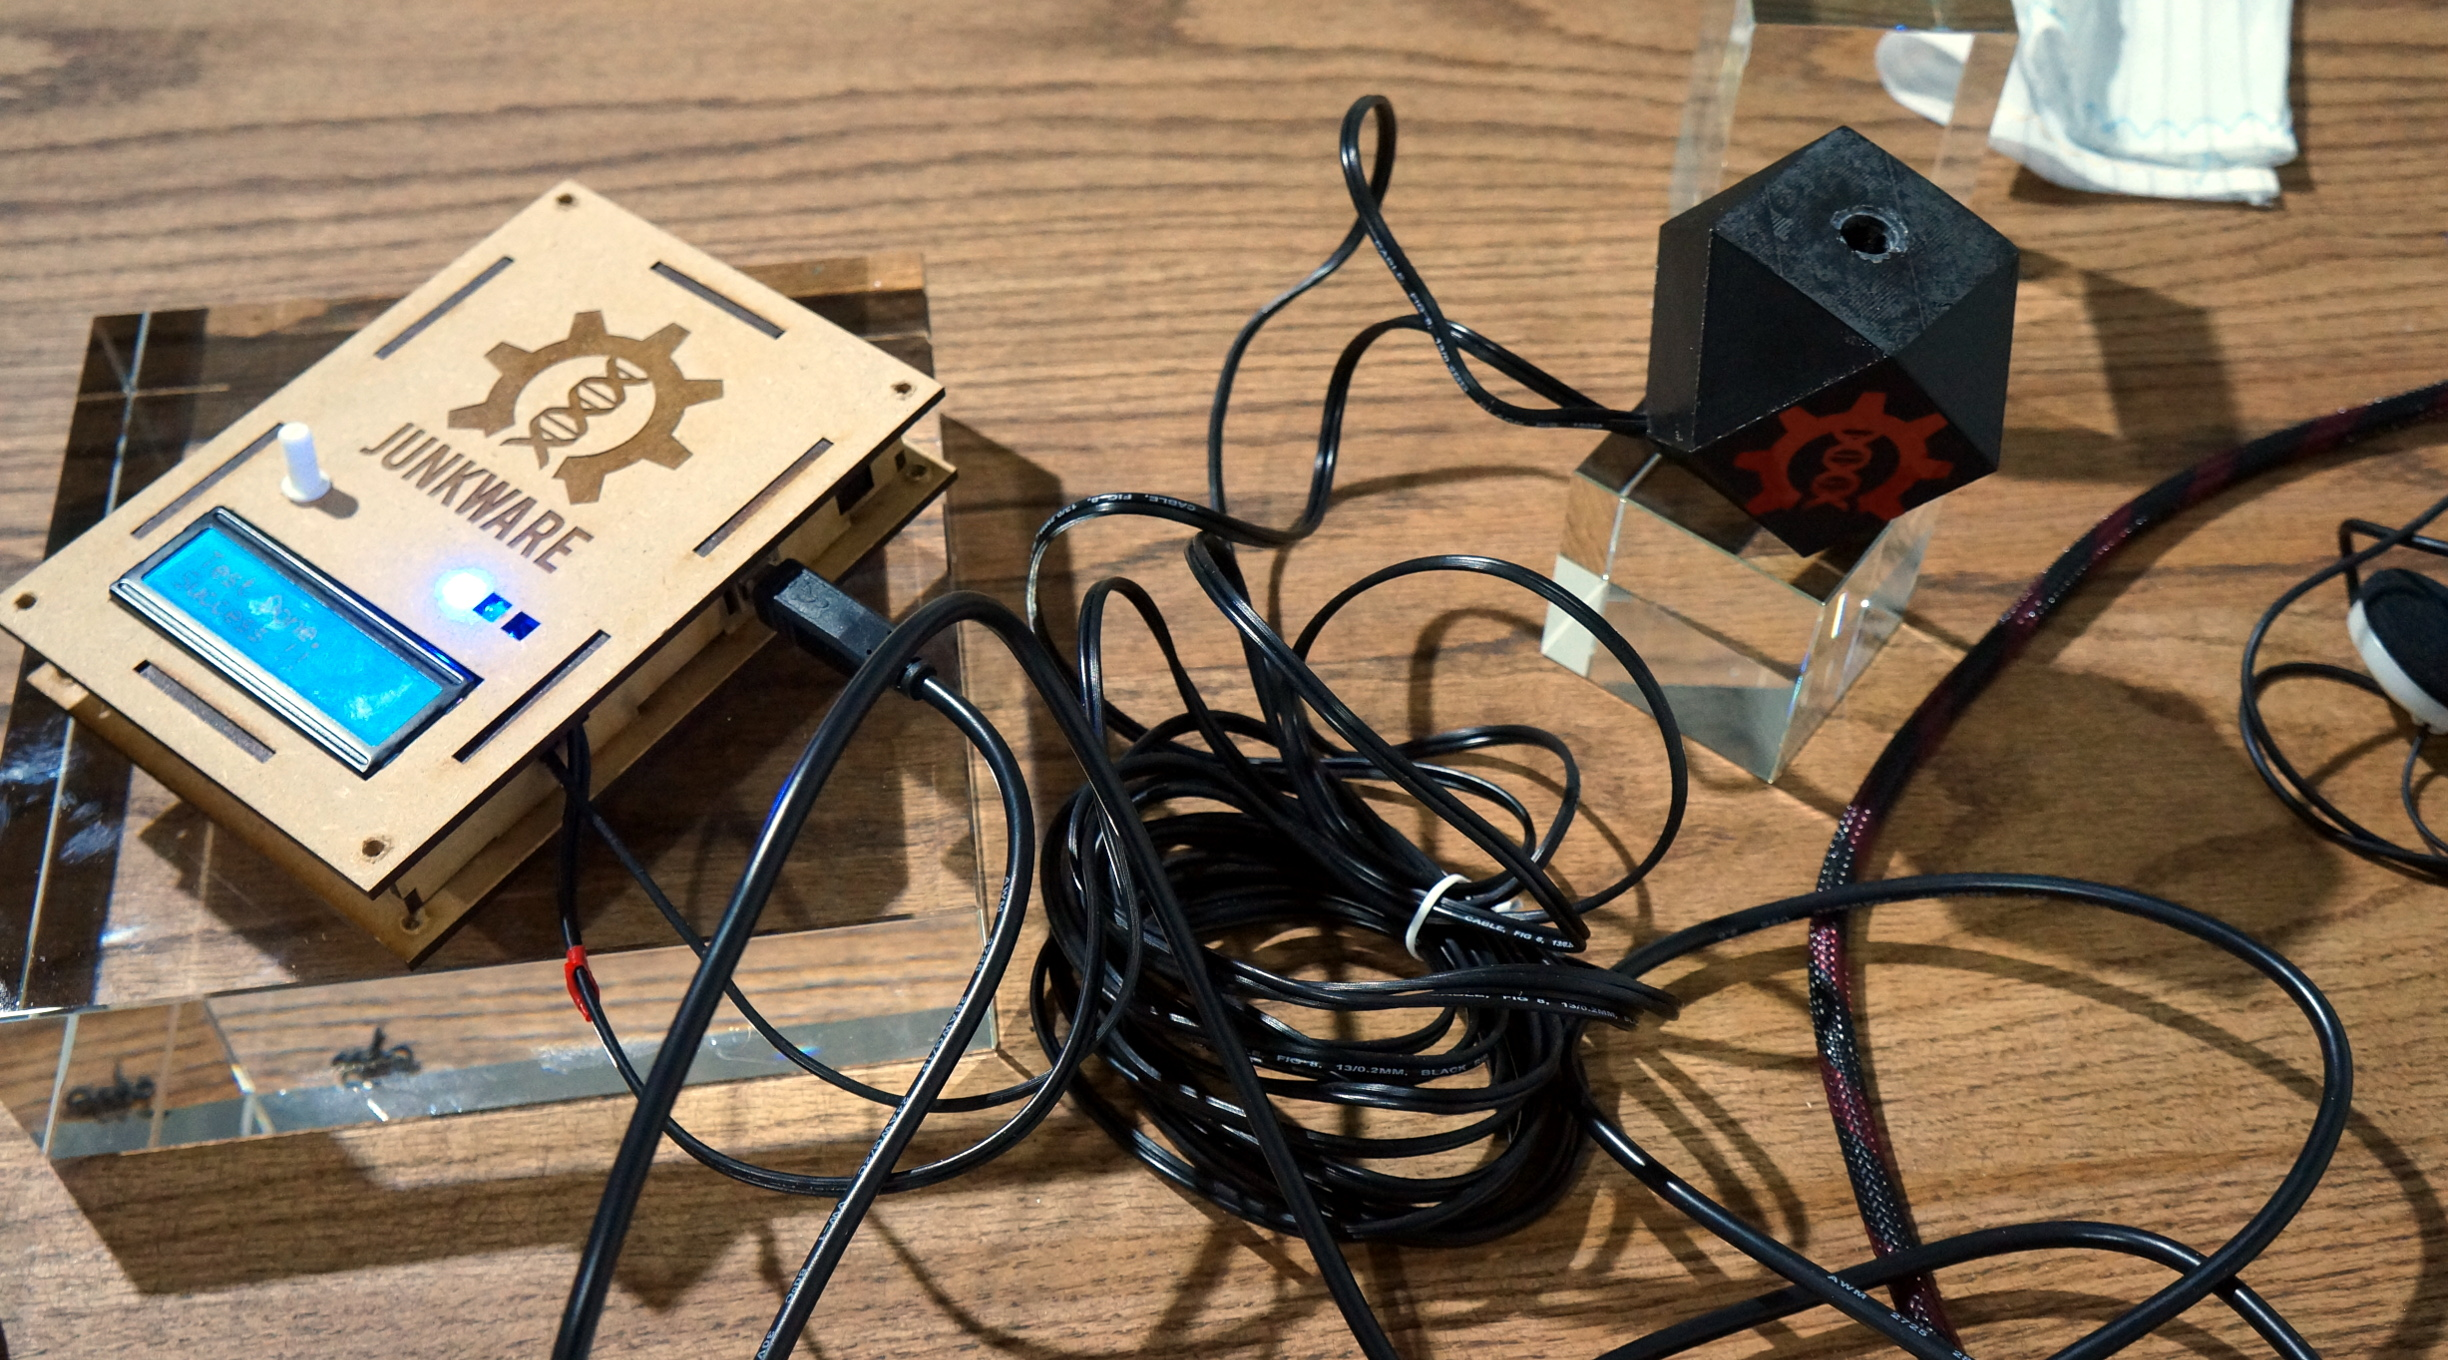
\includegraphics[width=5.5in,height=3.0547in]{images/junkware-img2.jpg}
\end{center}
{\centering\itshape
Caption : The junk sequencer -- Credits : Junkware (CC)
\par}


\bigskip

\subsection{Simulated behavior}
As part of the experiment, some features of the \textit{Junk Sequencer
}just recreates or simulates the attended behavior without having a
direct relationships with the biometric input. For instance, we display
correct values while monitoring the neural activity of the user but use
random values to generate the content. We also simulate the behavior of
a DNA sequencer with a home-made machine a random sequence generation.
In this work, we didn{\textquotesingle}t intend to use technology as a
endeavor but as a main component of a larger performance
setup\footnote{All code is avalilable at :
https://github.com/clemsos/junkware}.

\subsection[Inputs : Oxymeter, EEG and (fake) DNA sequencer]{Inputs :
Oxymeter, EEG and (fake) DNA sequencer}
The first form of input for the \textit{Junk Sequencer }is a DNA
sequence. The device is made of a 3D-printed shape with a slot to host
a pipette, a case including an LCD screen and a few led and a basic
step-motor that recreates the sound and centrifuge movement of the
sequencing. Connected to a computer through a micro-controller, this
device once activated will initialize the creation of a new fictional
object.\textit{ }The second form of input for the \textit{Junk
Sequencer }is an electroencephalographic (EEG) headset that interprets
the user{\textquoteright}s neural activity. The third form of input is
an oxymeter that gather pulse and heartbeat by being plugged on the
user{\textquotesingle}s finger.

\subsection[Content : Data \& Generators]{Content : Data \& Generators}
Once a new object is initiated, the machine will generate a new batch of
content from different existing data\footnote{All data is available
here : https://github.com/clemsos/junkware-data}. First, a new DNA
sequence will be created by adding randomly the four letters ACGT to
form a string of 4028 characters. \ Then we will apply some A-T
mutation to the newly formed protein using a frequency of 0.066\%. The
result will be stored in the database. The second important step will
be the creation of the textual description of the object using Natural
Language Generation (NLG). The description is creating by applying a
Markov chain algorithm to a training set of 10 documents selected
randomly from a large database of patents [Li2014]. The user can
regenerate multiple titles, abstracts and features definitions through
the interface and save its favorite result. The third important step is
the random choice of a file within a vast corpus of molecule
description from the World Protein Bank. The last step is a generation
of a set of numeric values to create 3D shape based on the
super-formula [Gielis2004]. The super-formula is a mathematical model
that allows to create and modify a coherent 3D shape by simple
geometric operations. Once we have created all those different data, we
can now represent each step of formation of our fictional object in the
user interface.

\subsection[Interface : Web Server \& Visualization ]{Interface : Web
Server \& Visualization }
The interface is based on HTML5 \& Javascript and is accessed through a
web browser. Communication with the data is assured with web sockets
and request to a web server. The real-time visualization of the
biometric data acquired through the different devices is based on d3.js
[Bostock2011]. The visualization of the molecule is based on Glmol
[Nakane2014]. The user interface allows the user to tweak and modify
different values obtained during the initialization phase. For
instance, the 3D model can be changed completely (shape, textures,
colors).


\bigskip



\begin{center}
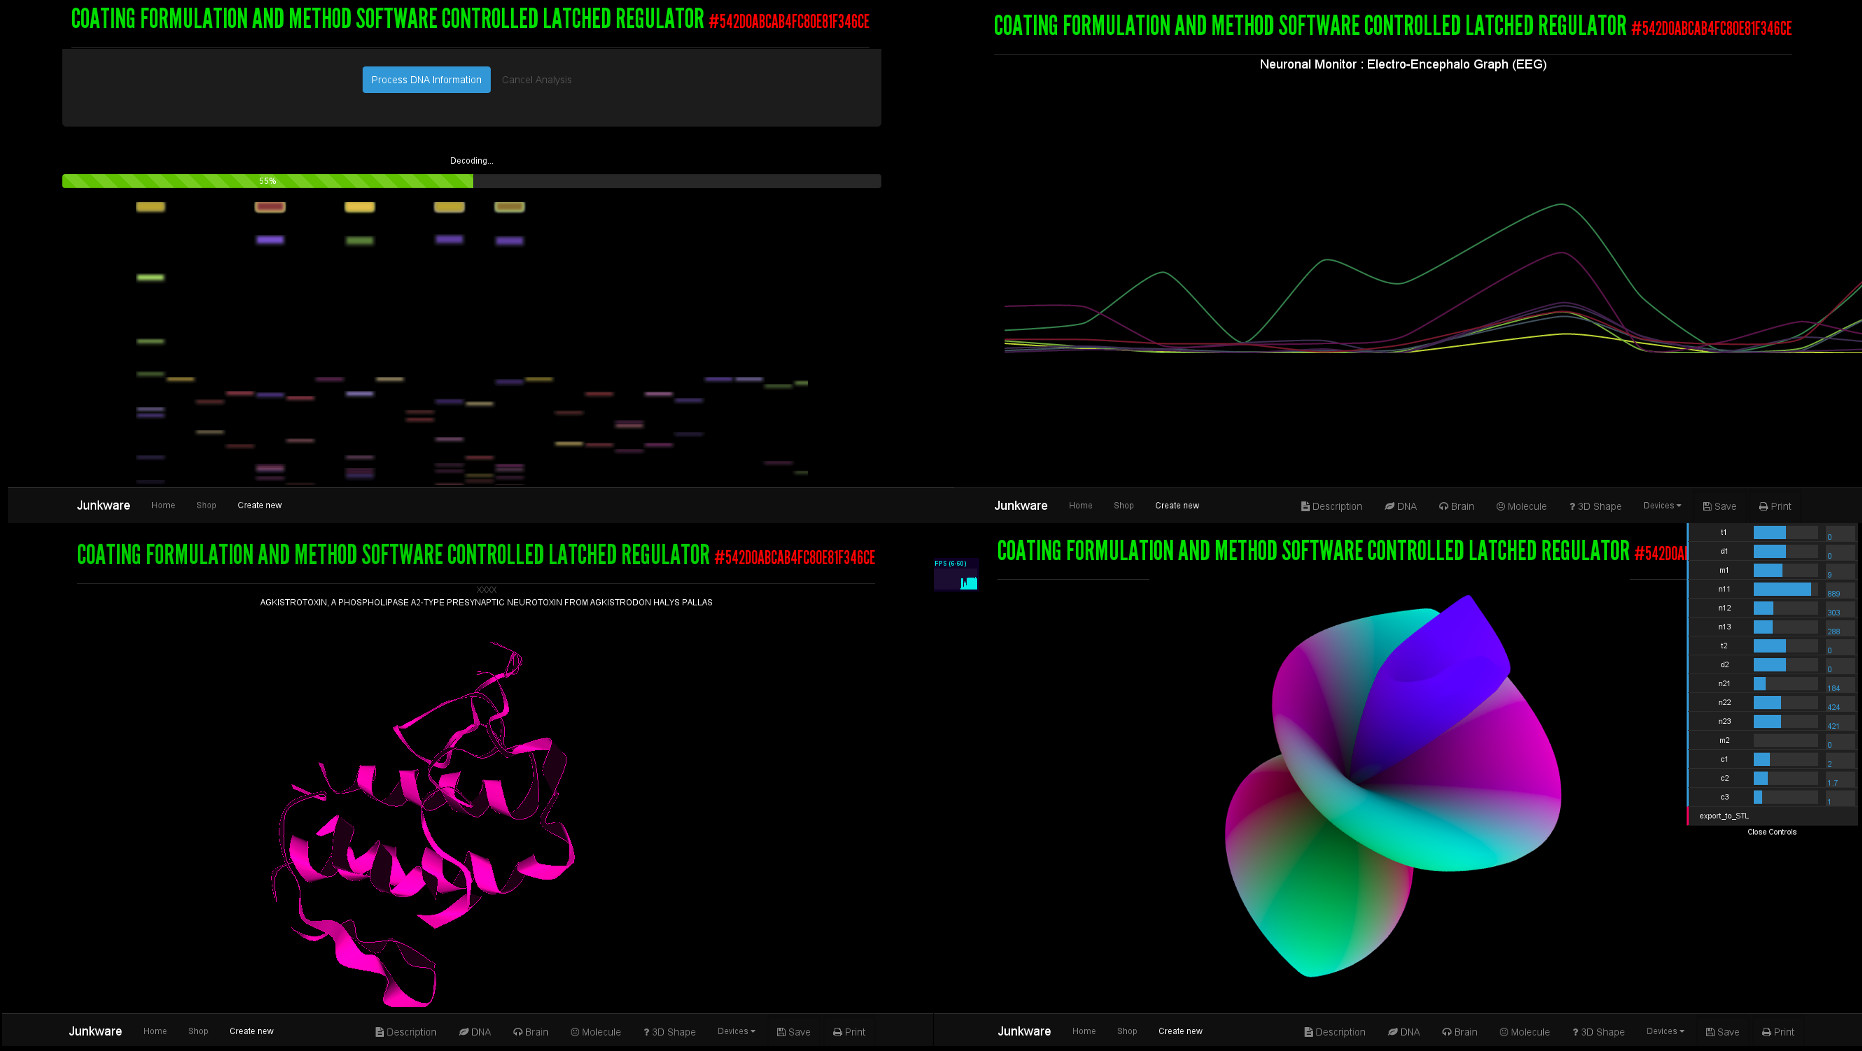
\includegraphics[width=6.9252in,height=3.9091in]{images/junkware-img3.jpg}
\end{center}
{\centering
Caption : The user interface showing a molecule and a randomly selected
title. 
\par}

{\centering
Screenshot taken on January 19, 2015 -- Credits : Junwkare.
\par}


\bigskip

\section[Play : the digital farce]{Play : the digital farce}
\subsection{The outstanding achievements of Pr. Roger Lafleche}
The first exhibition of the work took place during a technology fair
outdoor in Knowedlge Innovation Center in Shanghai, China. In our
installation, the professor Roger Lafleche, supposedly the inventor of
our machine, is the main character. Introduced as a great scientist, he
interacts with the audience through the several assistants that are
promoting his work during the installation. Only the ones who get
involved into the pseudo-scientific experiment get to talk to him.
Nevertheless, people can appreciate its scientific papers that have
been generated using SCIGen [Labbe2013] and even follow his work on
dedicated websites such as
\textit{A}\textit{cademia.edu}\footnote{https://independent.academia.edu/RogerLafleche}.


\subsection{Fortune-telling quarantine tent}
Inspired by both fortune-telling caravan and Ebola quarantine tents, the
main piece of the installation is the mobile lab. Defining a closed
space separated from the outside world, the lab can host 3 to 4 people
including the professor and its closest female assistant. The
participants that express the wish to test the installation are asked
to wait in line and signed the \textit{Terms of Contents. }The text of
this document has also been generated by mixing multiple existing terms
of contents and some others sources such as a divorce agreement. Once
the participant has signed it, he is allowed to enter the lab where he
has to quit his shoes and wear a full body medical suit. The entirety
of what is happening inside the tent is broadcast outside through a
video-surveillance system.


\bigskip



\begin{center}
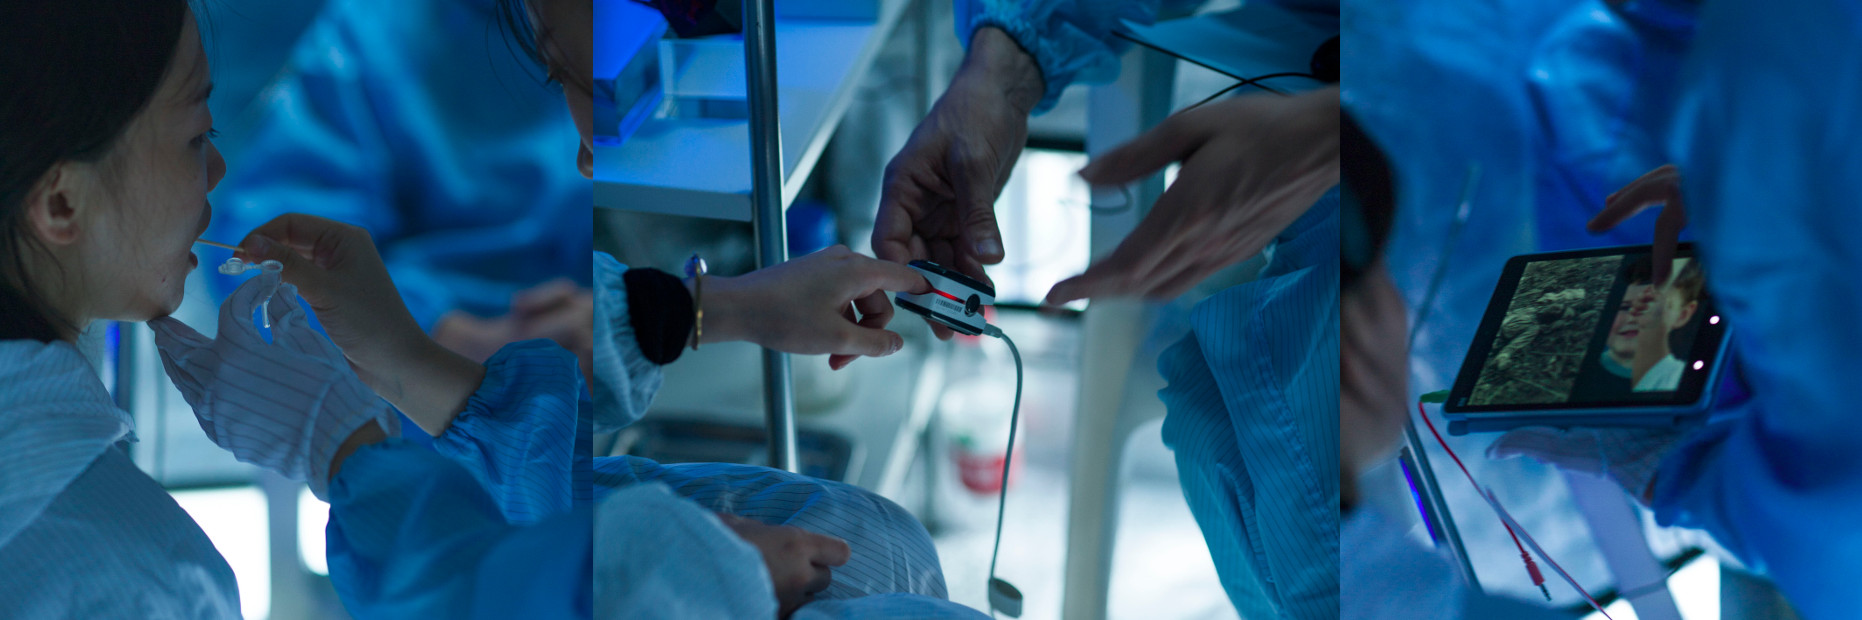
\includegraphics[width=6.9252in,height=2.3055in]{images/junkware-img4.jpg}
\end{center}
{\centering
Caption : Inside the tent, a user is submitted to different tests (DNA
sampling, oxymeter, images). Credits : Junkware (CC).
\par}


\bigskip

\subsection[Human input and generative sequence]{Human input and generative
sequence}
Here, he will meet the professor that will start processing the batch of
required tests, showing him all results on a computer screen. First, we
will record its DNA information by input a q-tip or a hair into the
\textit{Junk Sequencer}. To explain the very short time of the
sequencing (a few seconds only), we acknowledge that only information
about creativity are sequenced from the user{\textquotesingle}s DNA.
The next step is to show the molecular structure of our fictional
object by displaying the previously selected molecule on a screen. Once
this is done, we start monitoring the neural activity and hearth beat
of the user by placing devices onto him. Here he is shown with a
selection of images before being saddled with blind massaging glasses.
When he takes off the glasses, he can see the 3D shape representing the
object that was just generated from the previous sequence. Finally, the
textual description including name, abstract and details of the
features is displayed on the screen. 

\subsection{Rewarding collaborative work}
Once all the details about the structure and the complete description of
the object have been generated, the sequence ends and the user is
invited to exit the tent. A diploma is delivered to the user,
mentioning his unlimited ownership of the generated object and how
useful its contribution to science may be. This document named
\textit{Junwkare Honorary Credentials }\ is also an attestation of
participation that will be kept by the user. The shapes of the objects
produced during this process are 3D printed to create a growing gallery
of futuristic objects.


\bigskip

\section{Results }
More than fifty objects have been generated during the first
presentation of this work, which means \ than more than 50 people have
taken this experiment. For each of them, we have collected a sample of
saliva or a hair as well as their signature and some basic information
about their health. The character of the professor has been interviewed
about the stakes of its scientific work and some articles have been
published
online\footnote{\url{http://ima.nyu.sh/chinese-cyberculture/2014/10/24/junkware/},
consulted on February, 19 2015}. The team have been approached for
further collaborations by several companies during the exhibition. One
has even made an appointment with its boss at its headquarters -- the
meeting went well. 

\section{Discussions : Generative art and audience digital literacy}
This work offers a critical illustration of the self-fulfilling prophecy
of technological innovation. Collecting biometrics data by giving fake
credentials to a target audience is just one aspect of the
demonstration. One of the other obvious observation is the critical
role played by science in the success of such a grotesque experiment.
The facility to generate a technological simulacrum and provide
scientific validation through pseudo-papers and websites was a
relatively easy task. The white lab coat give final credits to what is
in reality non-achievements or maybe even worst. The fictional
environment we developed has allowed the non-innovative and useless
core processes to reach the status of a technological achievement.


\bigskip

Between the multiple people that have been attending this project, some
haven{\textquotesingle}t been tricked though. Most of the well-told
developers and scientists have catch easily the substantial amount of
fake information involved in the project. Still a large majority that
took it for granted and went along the lines of the scenario we
developed. We don{\textquotesingle}t intend here to show that it is
possible to mock and to cheat an audience. The magic involved in both
generative and scientific writing is a powerful tool that involves
singular forms of literacy to be understood. Our first intention was to
show the absurdity of an innovation process based on speculation about
an hypothetical future. Such processes eventually produces gibberish
and pipe dreams that may or may not turn into anything useful.
Ultimately the fundamental advantage that allow them to exist is this
vast gap in literacy regarding the making of technology.


\bigskip

\textit{Junwkare }is a formal experiment where fiction is meeting
performing arts, generative design and different ways of showing art.
Following the ideas of William James and its \textit{radical
empricism}, we think that knowledge is based on experience and feelings
before entering the space of representation. Therefore, we did not
intend to represent what bad practices of innovation may look like but
to become its grotesque reflection. Our original intention have been to
show the piece not in galleries but in scientific and technological
fairs, because we needed this context to make this experience exist.


\bigskip

Instead of looking at generative art as a specific expression, we have
tried here to bring it into a larger and broader form that projects it
to give it a real significance. We called literacy the capacity of a
specific group to bring technology into context to understand its
stakes and limits. Then we should now look forward to the new
byproducts of this literacy outside the domain of science or technology
and bring back art down to his role of drowning us into experience. As
stated by Artaud in the preface of its book \textit{The Theatre and Its
Double : }\textit{{\textquotedblleft}}\textit{I}\textit{f there is
still one hellish, truly accursed thing in our time, it is our artistic
dallying with forms, instead of being like victims burnt at the stake,
signaling through the }\textit{flames.{\textquotedblright}
}[Artaud1938] 

\section{Conclusion}
We have seen in this article the proposition made by the
\textit{Junkware} experimental project to bridge performing and
generative arts by providing a grotesque representation of innovation.
Originated in a reflection about futuristic objects, \textit{Junwkare
}introduces a setup where a fictional scientists, the professor Roger
Lafleche, has invented a machine called \textit{Junk Sequencer} to
generate description of forthcoming objects. Using different generative
algorithms, the machine shows visual and textual representations that,
once added into context become the ferment of a fictional object. In
this work ,we wanted to show how technological innovation itself uses a
discourse about the future to justify the endeavors of industrial
development. We also wanted to bring a more fundamental reflection
about the role of generative art in larger context, not only as a
formal exercise but also as a potential source of fiction and
reflection for the authors and their audience.


\bigskip

\section{Bibliography}
